\documentclass{beamer}

\mode<presentation>
{
  \usetheme{boxes}      
  \usecolortheme{default} 
  \usefonttheme{serif} 
  \setbeamertemplate{navigation symbols}{}
  \setbeamertemplate{caption}[numbered]
} 
\usepackage{tikz}
\setbeamercovered{highly dynamic}
\newcounter{saveenumi}
\newcommand{\seti}{\setcounter{saveenumi}{\value{enumi}}}
\newcommand{\conti}{\setcounter{enumi}{\value{saveenumi}}}
\renewcommand{\thefigure}{\thesection-\arabic{figure}}
\usetikzlibrary{shapes.geometric,calc,angles,positioning,intersections,quotes,decorations,babel,patterns,fit}
\usepackage{tkz-euclide}
\usetkzobj{all}
\usepackage[english]{babel}
\usepackage[utf8]{inputenc}
%\usepackage[T1]{fontenc}
\usepackage{graphics}
\usepackage{standalone}
\usepackage{gensymb}
\usepackage{listings}
\usepackage{amsmath}
\usepackage{amsmath}
\usepackage{hyperref}

\title[Your Short Title]{Assignment}
\author{Narendra}
\institute{IITH}
\date{}

\lstset{
%language=C,
frame=single, 
breaklines=true,
columns=fullflexible
}
\begin{document}
\begin{frame}
\titlepage
\end{frame}
\begin{frame}{Triangle}
{\textbf{Problem:1}\\Construct an isosceles right angled triangle ABC Right angled at C such AC = 6 . }
\begin{itemize}
\item \textbf{Solution:}
\end{itemize}
\textbf{Given} :\\$\Delta ABC$ is a Isosceles Right angle triangle i.e AC = BC = 6. \\
From the Baudhayana's theorem 
   \begin{align}
   AB^2 = AC^2 + BC^2 
   \end{align}
   then $AB^2 = 6^2 + 6^2 $\\
   $AB = \sqrt{72}$
the python code for  Figure 0-1 Isosceles triangle is codes/tri\_isoc.py\\
and the equivalent latex-tikz code  for Figure 0-2 is figs/tri\_isoc.tex
\end{frame}
\begin{frame}{}
\begin{figure}[!ht]
	\begin{center}
\includegraphics[width=0.8\columnwidth]{./figs/tri_isosc.eps}
	\end{center}
	\caption{Isosceles triangle}
	\label{fig:tri_Isosceles}	
\end{figure}
\end{frame}
\begin{frame}{}
\begin{figure}[!ht]
	\begin{center}
		\resizebox{0.6\columnwidth}{!}{\begin{tikzpicture}[scale=1]

%Triangle sides
\def\a{6}


%Marking coordiantes

\coordinate [label=above:$A$] (A)at (0,\a);
\coordinate [label=right:$B$] (B)at (\a,0);
\coordinate [label=left:$C$]  (C)at (0,0);

%Drawing triangle ABC
\color{blue}
\draw (A) -- node[right] {$\textrm{$\sqrt{72}$}$} (B);
\color{black}
\draw (B) -- node[below] {$\textrm{6}$} (C) -- node[right,,xshift=2mm] {$\textrm{6}$} (A);

%Drawing and marking angles
\tkzMarkAngle[fill=blue!40,size=0.5cm,mark=](A,B,C)
\tkzMarkRightAngle[fill=blue!20,size=.3](A,C,B)
\tkzLabelAngle[pos=-0.65](A,C,B){$$}
\end{tikzpicture}
}
	\end{center}
	\caption{Isosceles triangle}
	\label{fig:tri_Isosceles}	
\end{figure}
\end{frame}
\begin{frame}
\textbf{Coordinates to construct an Isosceles triangle:}
\begin{enumerate}
\item Construct a Isosceles triangle ABC which is right angled at C with a = b = 6.
\item Direction vector m is equals to A-B.
\item The vertices of $\Delta$ABC are A = $\begin{pmatrix} 0\\6 \end{pmatrix}$, B = $\begin{pmatrix} 6\\0 \end{pmatrix}$, C = $\begin{pmatrix} 0\\0 \end{pmatrix}.$ 
\end{enumerate}
\url{https://github.com/Narendrapulipati/geometry/blob/master/figs/tri_isoc.tex}
\url{https://github.com/Narendrapulipati/geometry/blob/master/codes/tri_isosc.py}
\end{frame}
\begin{frame}
{\textbf{Problem:2}\\AD is a median of a $\Delta$ABC and AM $\perp$ BC.\\
Prove that : \\
(i) AC$^2$ = AD$^2$ + BC.DM + $\left[\frac{BC}{2}\right]^2$,\\
(ii) AB$^2$ = AD$^2$ - BC.DM + $\left[\frac{BC}{2}\right]^2$,\\
(iii) AC$^2$ + AB$^2$ = 2AD$^2$ + $\frac{1}{2}$ BC$^2$.}
\begin{itemize}
\item \textbf{Solution:}
\end{itemize}
\textbf{Given:}\\
ABC is a Triangle AD is a median of $\Delta$ABC and AM $\perp$ BC.
\begin{align}
BD = CD = \frac{1}{2} BC
\end{align}
\textbf{Proof:}
(i) AC$^2$ = AD$^2$ + BC.DM + $\left[\frac{BC}{2}\right]^2$\\
\end{frame}
\begin{frame}
From Baudhayana's theorem $\Delta$AMD
\begin{align}
AD^2 = AM^2 + DM^2
\end{align}
From $\Delta$AMC
\begin{align}
AC^2 = AM^2 + CM^2
\end{align}
By subtracting Equation (3) from (4)\\
we get,\\ 
AC$^2$ - AD$^2$ = AM$^2$ + CM$^2$ - AM$^2$ - DM$^2$\\
AC$^2$ - AD$^2$ = CM$^2$ - DM$^2$\\
AC$^2$ = AD$^2$ + CM$^2$ - DM$^2$\\ 
putting CM = CD + DM \\ 
\enspace
AC$^2$ = AD$^2$ + (CD + DM)$^2$ - DM$^2$\\ 
AC$^2$ = AD$^2$ + CD$^2$ + DM$^2$ + 2.CD.DM - DM$^2$\\
AC$^2$ = AD$^2$ + CD$^2$ + 2.CD.DM\\
putting CD = $\frac{1}{2}$ BC from Equation (2)\\
AC$^2$ = AD$^2$ + $\left[\frac{1}{2} BC\right]^2 + 2\left[\frac{1}{2} BC\right].DM$
\end{frame}
\begin{frame}
\begin{align}
AC^2 = AD^2 + BC.DM + \left[\frac{BC}{2}\right]^2
\end{align}
(ii) AB$^2$ = AD$^2$ - BC.DM + $\left[\frac{BC}{2}\right]^2$,\\
By Applying Baudhayana's theorem $\Delta$AMB \\
we get 
\begin{align}
AB^2 = AM^2 + BM^2
\end{align}
and for $\Delta$AMD 
\begin{align}
AD^2 = AM^2 + DM^2
\end{align}
subtracting Equation (7) from (6) we get,\\
AB$^2$ - AD$^2$ = AM$^2$ + BM$^2$ -(AM$^2$ + DM$^2$)\\
AB$^2$ - AD$^2$ = AM$^2$ + BM$^2$ -AM$^2$ - DM$^2$
\begin{align}
AB^2 = AD^2 + BM^2 - DM^2
\end{align}
\end{frame}
\begin{frame}
By substituting BM = BD - DM\\ \enspace
AB$^2$ = AD$^2$ + (BD - DM)$^2$ - DM$^2$\\\enspace
= AD$^2$ + BD$^2$ + DM$^2$ - 2.BD.DM - DM$^2$\\
AB$^2$ = AD$^2$ + BD$^2$ - 2.BD.DM\\
put BD = $\frac{1}{2}$ BC from Equation (2)\\
AB$^2$ = AD$^2$ + $\left[\frac{1}{2} BC\right]^2 - 2.\left[\frac{1}{2} BC\right].DM$\\\enspace
= AD$^2$ + $\left[\frac{BC}{2}\right]^2 - BC.DM$
\begin{align}
AB^2 = AD^2 - BC.DM + \left[\frac{BC}{2}\right]^2
\end{align}
(iii) AC$^2$ + AB$^2$ = 2AD$^2$ + $\frac{1}{2}$ BC$^2$\\
By adding Equation (5) and (9) we get,\\
AC$^2$ + AB$^2$ = AD$^2$ + BC.DM + $\left[\frac{BC}{2}\right]^2 + AD^2 - BC.DM + \left[\frac{BC}{2}\right]^2$ \\
AC$^2$ + AB$^2$ = 2AD$^2$ + $2\left[\frac{BC^2}{4}\right]$
\begin{align}
AC^2 + AB^2 = 2AD^2 + \frac{1}{2} BC^2.
\end{align}
\end{frame}
\begin{frame}{}
the python code for  Figure 0-3 is codes/tri\_median.py\\
and the equivalent latex-tikz code for Figure 0-4 is figs/tri\_median.tex
\begin{figure}[!ht]
	\begin{center}
\includegraphics[width=0.8\columnwidth]{./figs/tri_median.eps}
	\end{center}
	\caption{}
	\label{}	
\end{figure}
\end{frame}
\begin{frame}{}
\begin{figure}[!ht]
	\begin{center}
		\resizebox{0.6\columnwidth}{!}{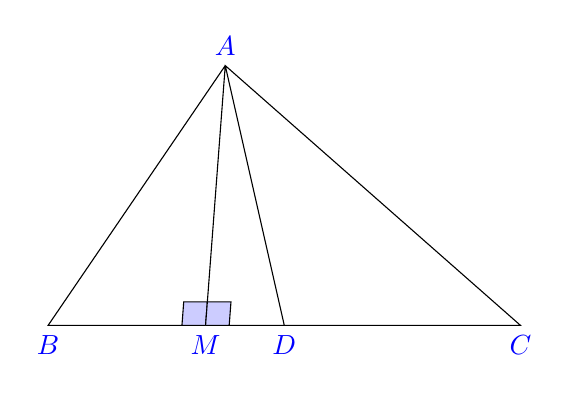
\begin{tikzpicture}[scale=1]

%Triangle sides
\def\a{2.25}
\def\b{3}
\def\c{6}
\def\d{2}
\def\e{3.3}
%Marking coordiantes
\color{blue}
\coordinate [label=above:$A$] (A) at (\a,\e);
\coordinate [label=below:$B$] (B) at (0,0);
\coordinate [label=below:$C$] (C) at (\c,0);
\coordinate [label=below:$D$] (D) at (\b,0);
\coordinate [label=below:$M$] (M) at (\d,0);

%Drawing triangle ABC
\color{black}
\draw (A) -- node[right] {$\textrm{}$} (B) -- node[below] {$\textrm{}$} (C) -- node[right,,xshift=2mm] {$\textrm{}$} (A)-- node[below] {$\textrm{}$} (M) (A)-- node[below] {$\textrm{}$} (D);

%Drawing and marking angles
\tkzMarkRightAngle[fill=blue!20,size=.3](A,M,B)
\tkzLabelAngle[pos=0.65](A,M,B){$ $}
\tkzMarkRightAngle[fill=blue!20,size=.3](A,M,C)
\tkzLabelAngle[pos=0.65](A,M,C){$ $}

\end{tikzpicture}
}
	\end{center}
	\caption{}
	\label{}	
\end{figure}
\end{frame}
\begin{frame}
\textbf{Coordinates of Triangle:}
\begin{enumerate}

\item Construct a $\Delta$ABC with median D and AM $\perp$ BC with a = 2.25, b = 3.3, c = 6 and D = $\frac{B+C}{2}$ = $\begin{pmatrix} 3\\0 \end{pmatrix}.$
\item  AM is the altitude of $\Delta$ABC.\\
\item A = $\begin{pmatrix} b\\a \end{pmatrix}$, B = $\begin{pmatrix} 0\\0 \end{pmatrix}$, C = $\begin{pmatrix} c\\0 \end{pmatrix}$ 
\end{enumerate}
\url{https://github.com/Narendrapulipati/geometry/blob/master/codes/tri_median.py}
\url{https://github.com/Narendrapulipati/geometry/blob/master/figs/tri_median.tex}
\end{frame}

\begin{frame}
{\textbf{Problem:3}\\In $\Delta$ABC, D and E are two points on BC such that BD = DE = EC. Show that ar(ABD) = ar(ADE) = ar(AEC).}
\begin{itemize}
\item \textbf{Solution:}
\end{itemize}
\textbf{Given:}\\
$\Delta$ABC where DE = DB = EC\\
Prove ar(ABD) = ar(ADE) = ar(AEC) \& take AL = Altitude of $\Delta$ABC\\
 Area of $\Delta$ ABC \begin{align}= \frac{1}{2}\times BD \times AL  \end{align}
 Area of $\Delta$ ADE \begin{align} = \frac{1}{2}\times DE \times AL \end{align}
\end{frame}
\begin{frame}
Area of $\Delta$ AEC \begin{align}= \frac{1}{2}\times EC \times AL \end{align}
By solving Equations (11), (12) we get,\\
$\frac{1}{2}\times$ BD $\times$ AL = $\frac{1}{2}\times$ DE $\times$ AL,\\ 
BD = DE. \\\enspace
By solving Equations (12), (13) we get,\\
$\frac{1}{2}\times$ BD $\times$ AL = $\frac{1}{2}\times$ EC $\times$ AL,\\
BD = EC. \\
from solving equations (11),(12) and (13) \\
BD = DE = EC\\\enspace
then, ar(ABD) = ar(ADE) = ar(AEC).\\\enspace
the python code for  Figure 0-5 is codes/tri\_area.py\\
and the equivalent latex-tikz code for Figure 0-6 is tri\_area.tex
\end{frame}
\begin{frame}{}
\begin{figure}[!ht]
	\begin{center}
\includegraphics[width=0.8\columnwidth]{./figs/tri_area.eps}
	\end{center}
	\caption{}
	\label{}	
\end{figure}
\end{frame}
\begin{frame}{}
\begin{figure}[!ht]
	\begin{center}
		\resizebox{0.8\columnwidth}{!}{\begin{tikzpicture}[scale=1]

%Triangle sides
\def\a{6}
\def\b{4}
\def\c{2}
\def\d{3}
\def\e{5}
%Marking coordiantes
\color{blue}
\coordinate [label=above:$A$] (A) at (\d,\e);
\coordinate [label=below:$B$] (B) at (0,0);
\coordinate [label=below:$C$] (C) at (\a,0);
\coordinate [label=below:$D$] (D) at (\c,0);
\coordinate [label=below:$E$] (E) at (\b,0);

%Drawing triangle ABC
\color{black}
\draw (A) -- node[right] {$\textrm{}$} (B) -- node[below] {$\textrm{}$} (C) -- node[right,,xshift=2mm] {$\textrm{}$} (A)-- node[below] {$\textrm{}$} (E) (A)-- node[below] {$\textrm{}$} (D) ;
\end{tikzpicture}
}
	\end{center}
	\caption{}
	\label{}	
\end{figure}
\end{frame}
\begin{frame}
\textbf{Coordinates of  Triangle:}
\begin{enumerate}
\item Construct triangle ABC and ADB and AEC with a = 5, b = 6, c = 3.
\item where D = $\frac{B+E}{2}$ and E = $\frac{D+C}{2}$.
\item The vertices of $\Delta$ABC are A = $\begin{pmatrix} c\\a \end{pmatrix}$, B = $\begin{pmatrix} 0\\0 \end{pmatrix}$, C = $\begin{pmatrix} b\\0 \end{pmatrix}.$ 
\end{enumerate}
\url{https://github.com/Narendrapulipati/geometry/blob/master/codes/tri_area.py}
\url{https://github.com/Narendrapulipati/geometry/blob/master/figs/tri_area.tex}
\end{frame}
\begin{frame}{Miscellaneous}
{\textbf{Problem:4}\\
The angle of elevation of the top of a tower from a point on the ground, which is 30m away from the foot of the tower, is $30\degree$. Find the height of the tower.}
\begin{itemize}
\item \textbf{Solution:}
\end{itemize}
\textbf{Given:}\\
Consider AB is the Tower\\
and C is the Elevation of the Tower \\
B is the foot of the Tower\\
CB = 30m\\
Angle of Elevation = $30\degree$ and $\angle$ ABC = 90$\degree$\\
We need to find AB (or) Hight of the Tower?\\
Consider the $\Delta$ABC \enspace 
\begin{align}
\tan C = \frac{Opposite}{Adjcent}
\end{align}
\end{frame}
\begin{frame}
i.e $\tan 30\degree = \frac{AB}{BC}$\\
AB = $\frac{30}{\sqrt{3}} = 10\sqrt{3}$
then,\\
AB = $10\sqrt{3}$m,\\
BC = 30m,\\
From the Baudhayana's theorem 
   \begin{align}
   AC^2 = AB^2 + BC^2 
   \end{align}
   then AC$^2$ = 30$^2$ + $(10\sqrt{3})^2$\\
   AC = $\sqrt{1200}.$\\
the python code for  Figure 0-7 is codes mis\_ex.py\\
and the equivalent latex-tikz code for Figure 0-8 is mis\_ex.tex
\end{frame}
\begin{frame}{}
\begin{figure}[!ht]
	\begin{center}
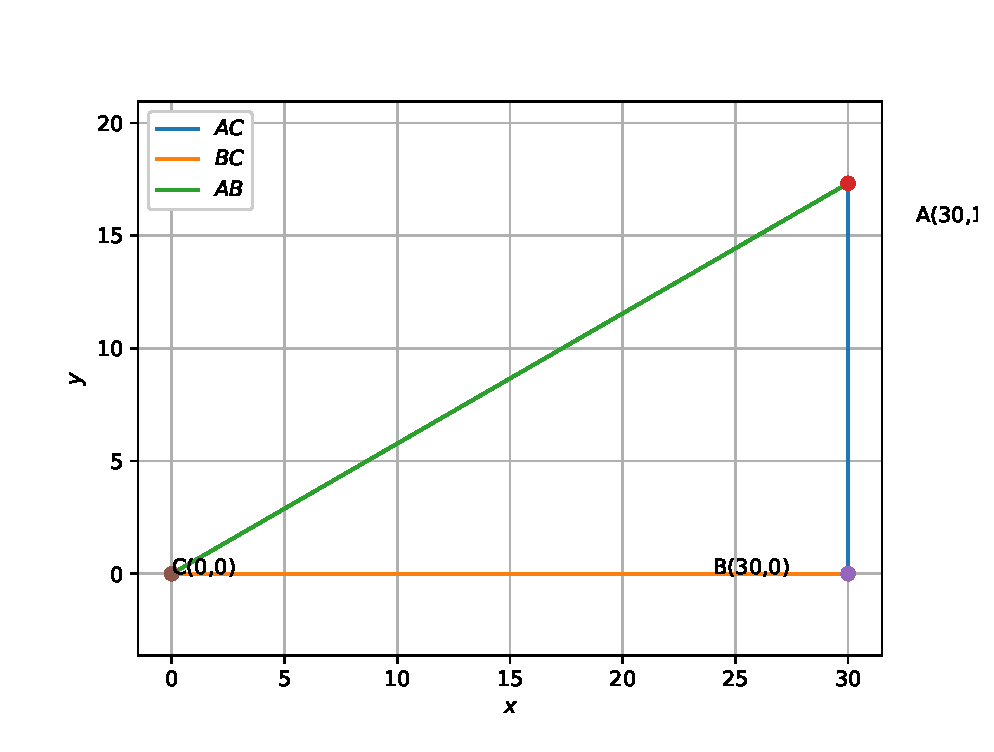
\includegraphics[width=0.8\columnwidth]{./figs/mis_ex.eps}
	\end{center}
	\caption{}
	\label{}	
\end{figure}
\end{frame}
\begin{frame}{}
\begin{figure}[!ht]
	\begin{center}
		\resizebox{0.8\columnwidth}{!}{
\begin{tikzpicture}[scale=1]

%Triangle sides
\def\a{30}
\def\c{17.34}

%Marking coordiantes
\coordinate [label=above:$A$] (A) at (\a,\c);
\coordinate [label=below:$B$] (B) at (\a,0);
\coordinate [label=left:$C$] (C) at (0,0);

%Drawing triangle ABC
\color{blue}
\draw (A) -- node[right] {$\textrm{10$\sqrt{3}$}$} (B);
\color{black}
\draw (B) -- node[below] {$\textrm{30}$} (C) -- node[above left,xshift=2mm] {$\textrm{$\sqrt{1200}$}$} (A);

%Drawing and marking angles
\tkzMarkAngle[fill=red!40,size=0.8cm,mark=](B,C,A)
\tkzMarkRightAngle[fill=blue!20,size=.3](A,B,C)
\tkzLabelAngle[pos=0.65](A,C,B)[right]{$30\degree$}

\end{tikzpicture}

}
	\end{center}
	\caption{}
	\label{}	
\end{figure}
\end{frame}
\begin{frame}
\textbf{Coordinates:}
\begin{enumerate}
\item Construct a triangle ABC which is right angled at B with a = 30, b = $10\sqrt{3}$ $\&$ C = 30$\degree$.
\item Direction vector m is equals to C-A.
\item The vertices of $\Delta$ABC are A = $\begin{pmatrix} a\\b \end{pmatrix}$, B = $\begin{pmatrix} a\\0 \end{pmatrix}$, C = $\begin{pmatrix} 0\\0 \end{pmatrix}.$ 
\end{enumerate}
\url{https://github.com/Narendrapulipati/geometry/blob/master/figs/mis_ex.tex}\\
\url{https://github.com/Narendrapulipati/geometry/blob/master/codes/mis_ex.py}
\end{frame}
\begin{frame}{Qudrilateral}
{\textbf{Problem:5}\\Construct a kite EASY if AY = 8, EY = 4 and SY = 6.}
\begin{itemize}
\item \textbf{Solution:}
\end{itemize}
\textbf{Given:}\\
AY = 8cm, EY = 6cm, SY = 7cm.\\
from the Quadrilaterel EASY\\
we know the upper two sides and lower two sides of a kite is equal\\ 
i.e EA = EY = 6cm and SA = SY = 7cm.\\

the python code for  Figure 0-9 is /codes/quad\_con.py\\
and the equivalent latex-tikz for Figure 0-10 is /figs/quad\_con.tex
\end{frame}
\begin{frame}
\textbf{Construction Of Quadrilateral:}\\
Consider the $\Delta$ AOE
\begin{align}
AE^2 = AO^2 + OE^2
\end{align}
$6^2 = 4^2$ + OE$^2$\\
OE = $\sqrt{20}$.\\
From the $\Delta$ AOS
\begin{align}
YS^2 = YO^2 + OS^2
\end{align}
$7^2 = 4^2$ + OS$^2$\\
OS = $\sqrt{33}.$\\
\end{frame}
\begin{frame}{}
\begin{figure}[!ht]
	\begin{center}
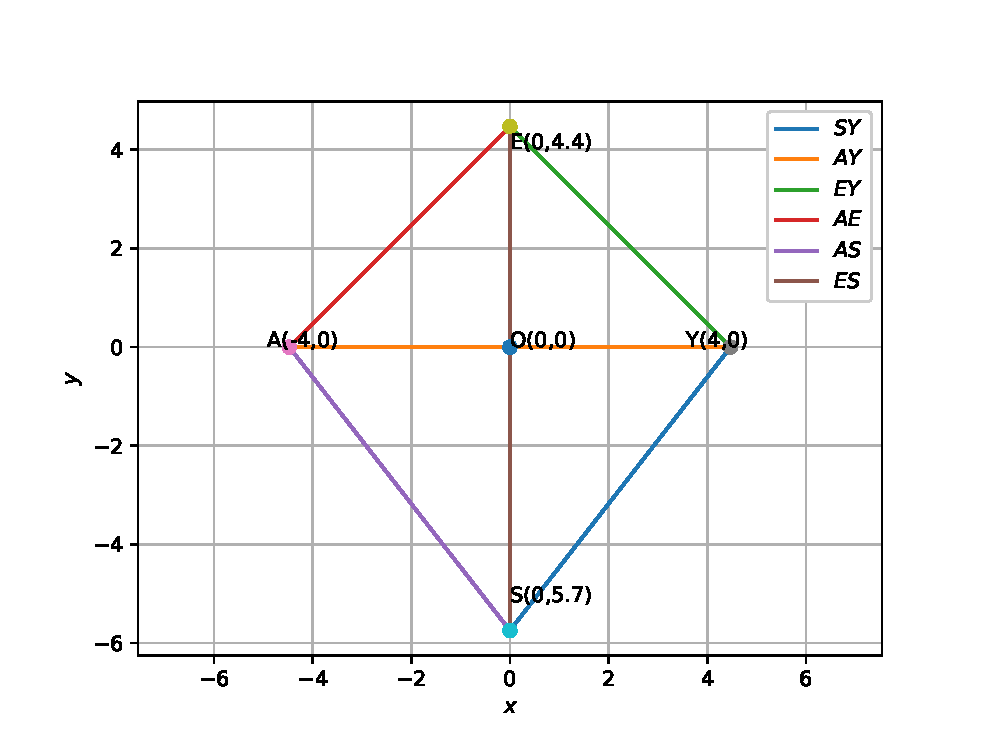
\includegraphics[width=0.8\columnwidth]{./figs/quad_con.eps}
	\end{center}
	\caption{Quadrilateral}
	\label{}	
\end{figure}
\end{frame}
\begin{frame}{}
\begin{figure}[!ht]
	\begin{center}
		\resizebox{0.6\columnwidth}{!}{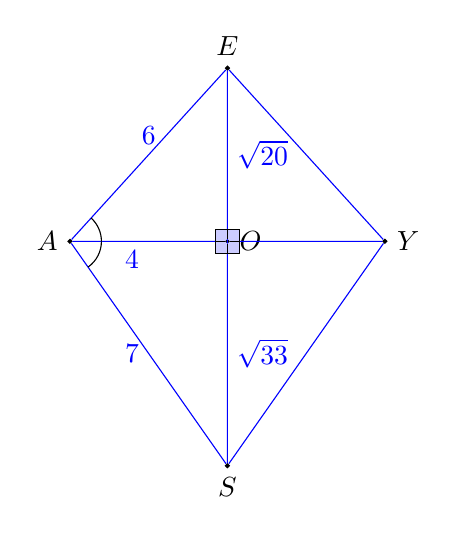
\begin{tikzpicture}
[scale=0.5,>=stealth,point/.style={draw,circle,fill = black,inner sep=0.5pt},]

%quadrilateral sides
\def\a{4.4}
\def\b{5.7}
\def\c{4}

%Labeling points
\node (E) at (0,\a)[point,label=above:$E$] {};
\node (A) at (-\c,0)[point,label=left:$A$] {};
\node (S) at (0,-\b)[point,label=below:$S$] {};
\node (Y) at (\c,0)[point,label=right:$Y$] {};
\node (O) at ($(A)!0.5!(Y)$)[point,label=right:$O$] {};
%Drawing Quadrilateral EASY
\color{blue}
\draw (E)--node[above] {$\textrm{6}$}(A)--node[left] {$\textrm{7}$}(S)--node[right] {$\textrm{}$}(Y)--node[right] {$\textrm{}$}(E)--node[right] {$\textrm{}$}(S)(A)--node[below left]{$\textrm{4}$}(O)--node[left]{$\textrm{}$}(Y)(O)--node[right]{$\textrm{$\sqrt{20}$}$}(E)(O)--node[right]{$\textrm{$\sqrt{33}$}$}(S);

%Drawing and marking angles
\color{black}
\tkzMarkAngle[fill=black!40,size=0.8cm,mark=](O,A,E)
\tkzMarkAngle[fill=black!40,size=0.8cm,mark=](S,A,O)
\tkzMarkRightAngle[fill=blue!20,size=.3](A,O,E)
\tkzMarkRightAngle[fill=blue!20,size=.3](Y,O,E)
\tkzMarkRightAngle[fill=blue!20,size=.3](A,O,S)
\tkzMarkRightAngle[fill=blue!20,size=.3](Y,O,S)
\end{tikzpicture}
}
	\end{center}
	\caption{Quadrilateral}
	\label{}	
\end{figure}
\end{frame}
\begin{frame}
\textbf{Coordinates of quadrilateral:}
\\
Construct a quadrilateral(Kite) EASY\\
\begin{enumerate}
\item A =$\begin{pmatrix} -4\\0 \end{pmatrix}$ and Y is $\begin{pmatrix}  4\\0 \end{pmatrix}$
\item O is taken as the origine i.e at $\begin{pmatrix} 0\\0 \end{pmatrix}$
\item The coordinates of E and S are  $\begin{pmatrix}  0\\ \sqrt{20} \end{pmatrix}$ $\begin{pmatrix} 0\\-\sqrt{33} \end{pmatrix}.$
\end{enumerate}
\url{https://github.com/Narendrapulipati/geometry/blob/master/codes/quad_con.py}
\url{https://github.com/Narendrapulipati/geometry/blob/master/figs/quad_con.tex}
\end{frame}
\begin{frame}
{\textbf{Problem:6}\\A rectangular park is to be designed whose breadth is 3m less then its length. Its area is to be 4square metres more than the area of a park that already been made in the shape of an isosceles triangle with its base as the breadth of the rectangular park and of altitude of 12m. Find its length and breadth.}
\begin{itemize}
\item \textbf{Solution:}
\end{itemize}
\textbf{Given:} A rectangualr park \\
breadth = length - 3\\
A Isosceles triangle\\
Altitude = Height = 12m\\
Area of rectangle = Area of triangle + 4\\
base of the triangle = breadth of the rectangular  park.\\
\end{frame}
\begin{frame}
from the Given we need to find  lenght, breadth, Area$_{rec},$ Area$_{tri}$ ?\\
 Area of the rectangle
\begin{align}
 = l \times b
 \end{align}
= $l(l - 3).$\\
Area of the triangle
\begin{align}
 = \frac{1}{2} \times b \times h
\end{align}
 = $\frac{1}{2} \times (l -3)\times 12 = 6(l - 3).$\\
from the Given Area$_{rec}$ = Area$_{tri}$ + 4\\
i.e \enspace
$l(l - 3) = 6(l - 3) + 4$\\
$l^2 + 9l + 14 = 0$ \\
$l = 7.$\\
then, Area$_{tri}$ = 6(7 - 3) = 24 m$^2$\\
Area$_{rec}$ = 7 $\times$ 4 = 28 m$^2$ (or) Area$_{rec}$ =  24 + 4 = 28 m$^2.$\\
the python code for  Figure 1-11 is codes/tri\_rect.py\\
and the equivalent latex-tikz code for Figure 1-12 is fig/tri\_rect.tex
\end{frame}
\begin{frame}{}
\begin{figure}[!ht]
	\begin{center}
\includegraphics[width=1\columnwidth]{./figs/tri_rect.eps}
	\end{center}
	\caption{}
	\label{}	
\end{figure} 
\end{frame}
\begin{frame}{}
\begin{figure}[!ht]
	\begin{center}
		\resizebox{0.3\columnwidth}{!}{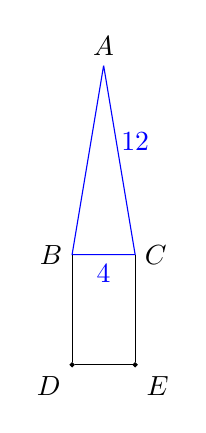
\begin{tikzpicture}
[scale=.2,>=stealth,point/.style={draw,circle,fill = black,inner sep=0.5pt},]

%Triangle sides
\def\a{4}
\def\b{7}
\def\c{3}
\def\d{2}
\def\e{19}

%Marking coordiantes
\color{black}
\coordinate [label=above:$A$] (A) at (\d,\e);
\coordinate [label=left:$B$] (B) at (0,\b);
\coordinate [label=right:$C$] (C) at (\a,\b);



%Drawing triangle ABC
\color{blue}
\draw (A) -- node[left] {$\textrm{}$} (B) -- node[below] {$\textrm{4}$} (C) -- node[above,,xshift=2mm] {$\textrm{12}$} (A);
\color{black}
\node (D) at (0, 0)[point,label=below left:$D$] {} ;
\node (E) at (\a, 0)[point,label=below right:$E$] {};

%Joining BD, CE and DE
\draw (B)--(D) ;
\draw (C)--(E);
\draw (D)--(E);

\end{tikzpicture}}
	\end{center}
	\caption{}
	\label{}	
\end{figure}
\end{frame}
\begin{frame}{}
\textbf{Coordinates:}
\begin{enumerate}
\item Take the point D as origin $\begin{pmatrix} 0\\0 \end{pmatrix}.$
\item E = $\begin{pmatrix} 4\\0 \end{pmatrix}.$
\item B = $\begin{pmatrix} 0\\7 \end{pmatrix}.$
\item Draw a line DB from the D to B.
\item C = $\begin{pmatrix} 4\\7 \end{pmatrix}.$
\item Join the all points of rectangle BCDE.\\
Then draw a triangle with the base of BC and with the altitude of A = 12.\\
\item A = $\begin{pmatrix} 2\\19 \end{pmatrix}.$
\item Join the all line segments of triangle ABC.  
\end{enumerate}
\end{frame}
\begin{frame}
\url{https://github.com/Narendrapulipati/geometry/blob/master/codes/tri_rect.py}
\url{https://github.com/Narendrapulipati/geometry/blob/master/figs/tri_rect.tex}
\end{frame}
\begin{frame}{Circle}
{\textbf{Problem:7}\\Let A and B be the centres of two circles of equal radii 3 such that each one of them passes through the centre of the other. Let them intersect at C and D. Is AB $\perp$ CD?}
\begin{itemize}
\item \textbf{Solution:}
\end{itemize}
\textbf{Given:}\\
Radious of circle A = B = 3cm .\\
C and D are the intersecting points.\\
AD = AC and BD = BC.\\
Radius of both circles are equal,\\
 therefore,\\
 AD = AC = BC = BD.\\
then ABCD form a Rhombus and the diagonals of rhombus bisects each other at 90\degree.\\
from the figure  AB $\perp$ CD.\\ 
the python code for  Figure 0-13 is codes/cir\_con.py\\
and the equivalent latex-tikz code for Figure 0-14 is cir\_con.tex
\end{frame}
\begin{frame}{} 
\begin{figure}[!ht]
	\begin{center}
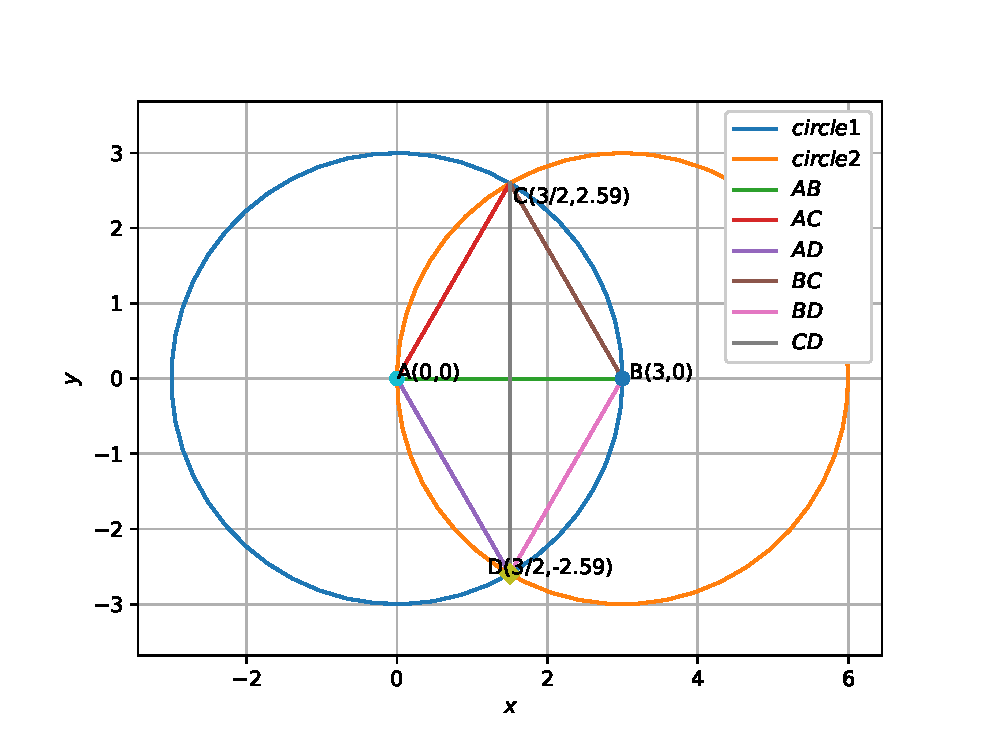
\includegraphics[width=0.8\columnwidth]{./figs/circle_con.eps}
	\end{center}
	\caption{Intersection of circles}
	\label{}	
\end{figure}
\end{frame}
\begin{frame}
\begin{figure}[!ht]
	\begin{center}
		\resizebox{0.8\columnwidth}{!}{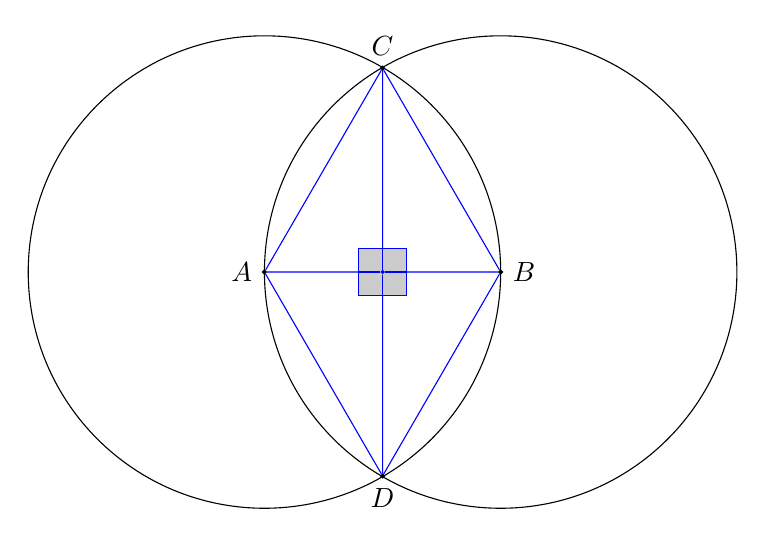
\begin{tikzpicture}
[scale=1,>=stealth,point/.style={draw,circle,fill = black,inner sep=0.5pt},]
%Inradius
\def\r{3} 
\node (A) at (0,0)[point,label=left:$A$] {};
\def\s{3} 
\node (B) at (3,0)[point,label=right:$B$] {};

%Drawing circle
\color{black}
\draw (A) circle (\r);
\draw (B) circle (\s);

%intersecting points
\def\a{1.5}
\def\b{2.59}
\color{black}
\node (C) at (\a,\b)[point,label=above:$C$] {};
\node (D) at (\a,-\b)[point,label=below:$D$] {};
\node (o) at (\a,0)[point,label=left:$o$] {};

%Drawing Rhombus
\color{blue}
\draw (A) -- node[left] {$\textrm{}$} (B) -- node[below] {$\textrm{}$} (C) -- node[right,,xshift=2mm] {$\textrm{}$} (A)-- node[below] {$\textrm{}$} (D)-- node[below] {$\textrm{}$} (B) (D)-- node[below] {$\textrm{}$} (C);
%Drawing the angles
\tkzMarkRightAngle[fill=black!20,size=.3](C,o,B)
\tkzMarkRightAngle[fill=black!20,size=.3](C,o,A)
\tkzMarkRightAngle[fill=black!20,size=.3](D,o,B)
\tkzMarkRightAngle[fill=black!20,size=.3](D,o,A)
\end{tikzpicture}}
	\end{center}
	\caption{Intersection of circles}
	\label{}	
\end{figure}
\end{frame}
\begin{frame}
\textbf{Coordinates of Circle:}
\begin{enumerate}
\item Construct two circles A and B which are intersecting at C and D.
\item A = $\begin{pmatrix} 0\\0 \end{pmatrix}$ ,B = $\begin{pmatrix} 3\\0 \end{pmatrix}.$
\item C = $\begin{pmatrix} p\\q \end{pmatrix} = \begin{pmatrix} \frac{3}{2}\\2.59 \end{pmatrix}$ ,
D = $\begin{pmatrix} p\\-q \end{pmatrix} = \begin{pmatrix} \frac{3}{2}\\-2.59 \end{pmatrix}.$\\
p and q are given as p = $\frac{c^2+b^2-a^2}{2c}$ = $\frac{3}{2}$ and\\
 q = $\sqrt{b^2-p^2} = 2.59$ (where a = b = c =3).
\end{enumerate}
\url{https://github.com/Narendrapulipati/geometry/blob/master/codes/cir_con.py}
\url{https://github.com/Narendrapulipati/geometry/blob/master/figs/circle_con.tex}
\end{frame}
\end{document}
